\subsection{Entstehung der Orbitaltheorie}
\label{subsec:entstehung_orbitaltheorie}

Die Schrödingergleichung\index{Schrödingergleichung} für das
Wasserstoffatom\index{Wasserstoffatom} liefert nicht nur bestimmte
Energiewerte, sondern auch die zugehörigen Wellenfunktionen\index{Wellenfunktion}.
Diese Wellenfunktionen beschreiben den quantenmechanischen Zustand
\index{Zustand!quantenmechanischer} des Elektrons\index{Elektron} im Atom.

Damit entsteht ein neues Bild des Atoms. Im bohrschen Atommodell
\index{bohrsches Atommodell} bewegt sich das Elektron noch auf festen Bahnen
\index{Bahn} um den Atomkern\index{Atomkern}. Diese Bahnen besitzen bestimmte
Radien und bestimmte Energien. Dieses Modell konnte einige Eigenschaften des
Wasserstoffatoms erklären, blieb aber letztlich ein Zwischenmodell.

In der Quantenmechanik gibt es solche festen Elektronenbahnen
\index{Elektronenbahn} nicht mehr. Das Elektron wird nicht durch eine Bahnkurve
beschrieben, sondern durch eine Wellenfunktion. Aus dem Betragsquadrat dieser
Wellenfunktion ergibt sich die Aufenthaltswahrscheinlichkeit
\index{Aufenthaltswahrscheinlichkeit} des Elektrons:

\begin{equation}
	\rho(\vec r) = |\psi(\vec r)|^2 .
	\label{eq:aufenthaltswahrscheinlichkeit_orbital}
\end{equation}

Dabei beschreibt \(\rho(\vec r)\)\index{Wahrscheinlichkeitsdichte} die
Wahrscheinlichkeitsdichte am Ort \(\vec r\). Orte mit großem Wert von
\(|\psi(\vec r)|^2\) sind Bereiche, in denen das Elektron mit hoher
Wahrscheinlichkeit gefunden wird. Orte mit kleinem Wert sind entsprechend
weniger wahrscheinlich.

Ein Orbital\index{Orbital}\index{Atomorbital} ist daher keine Bahn. Es ist ein
räumlicher Bereich, der durch die Wellenfunktion eines Elektrons bestimmt wird.
Anschaulich kann man ein Orbital als eine Form darstellen, innerhalb derer sich
das Elektron mit hoher Wahrscheinlichkeit befindet. Diese Darstellung ist aber
nur ein Bild für die Wahrscheinlichkeitsverteilung, nicht eine feste Oberfläche
oder eine materielle Hülle.
\FloatBarrier
\begin{PhysicsBox}[Bedeutung eines Orbitals]
	\label{box:bedeutung_orbital}
	Ein Orbital ist keine klassische Bahn eines Elektrons. Es beschreibt eine
	räumliche Wahrscheinlichkeitsverteilung, die aus der Wellenfunktion des
	Elektrons hervorgeht.
\end{PhysicsBox}

\FloatBarrier
\begin{figure}[H]
	\centering
	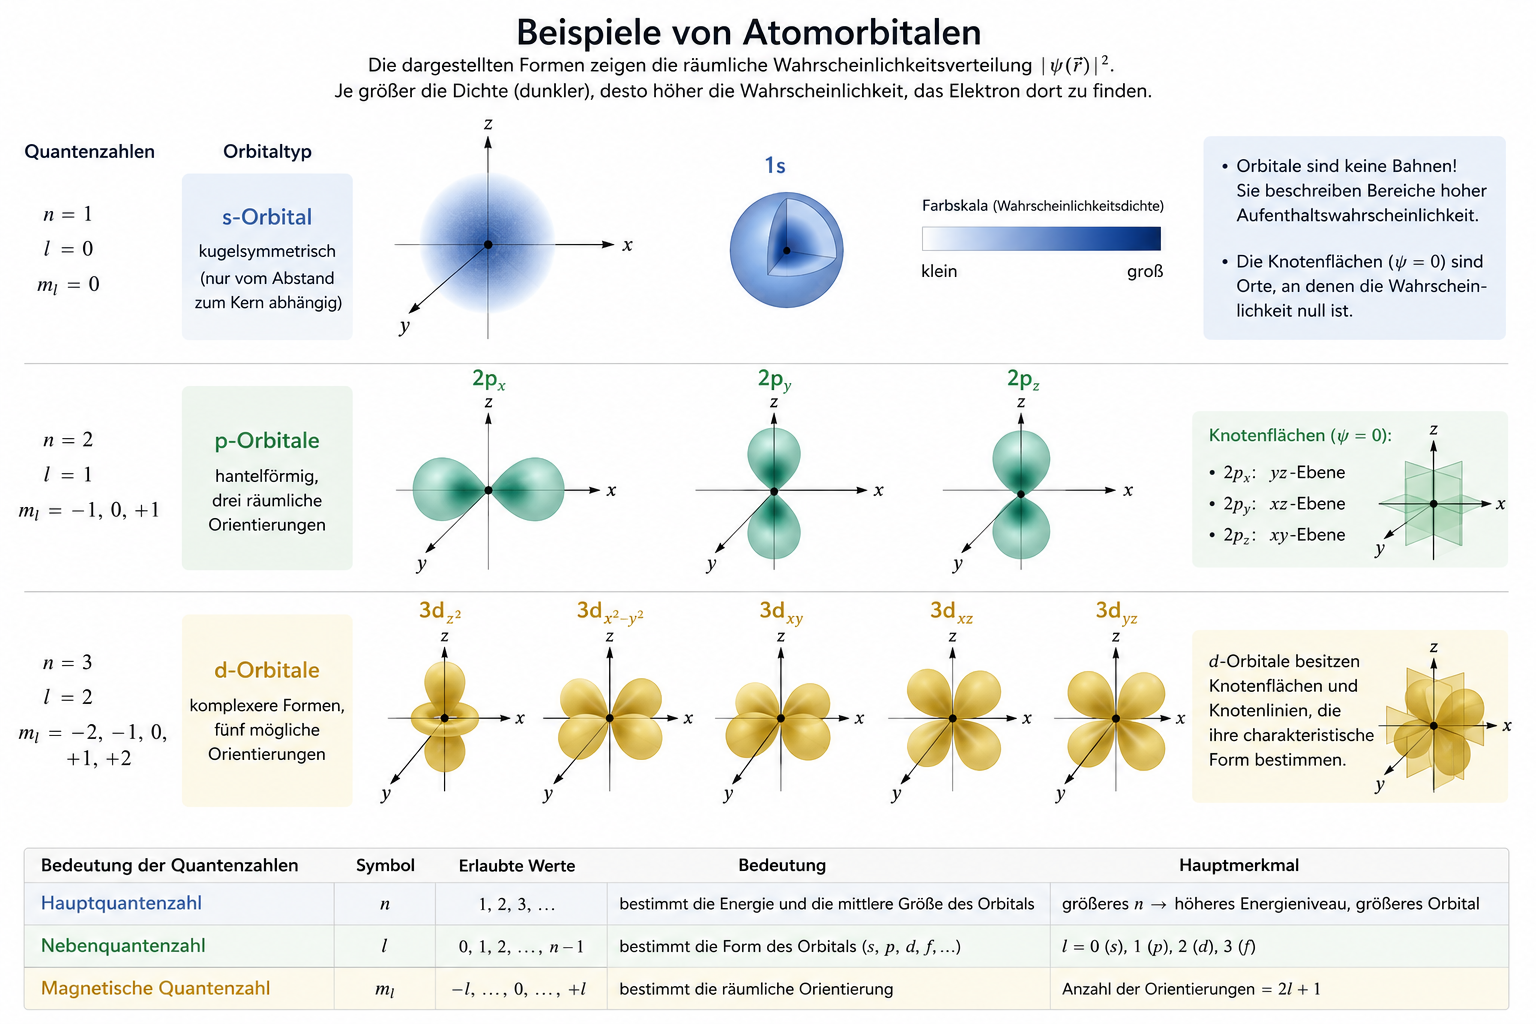
\includegraphics[width=\textwidth]{bilder/atomorbital}
	\caption{Beispiele von Atomorbitalen. Die dargestellten Formen zeigen die
		räumliche Wahrscheinlichkeitsverteilung \( |\psi(\vec r)|^2 \) eines
		Elektrons. Dunklere Bereiche entsprechen einer höheren
		Aufenthaltswahrscheinlichkeit.}
	\label{fig:atomorbitale_beispiele}
\end{figure}




Die Lösungen der Schrödingergleichung besitzen verschiedene räumliche Formen.

Die Lösungen der Schrödingergleichung besitzen verschiedene räumliche Formen.
Diese Formen werden durch Quantenzahlen\index{Quantenzahl} beschrieben. Für das
Wasserstoffatom treten vor allem drei Quantenzahlen auf: die Hauptquantenzahl,
die Nebenquantenzahl und die magnetische Quantenzahl.

Die Hauptquantenzahl\index{Hauptquantenzahl} \(n\) bestimmt im Wesentlichen das
Energieniveau\index{Energieniveau} und die räumliche Ausdehnung des Orbitals.
Je größer \(n\) ist, desto höher ist im Wasserstoffatom die Energie des Zustands
und desto weiter reicht das Orbital im Mittel vom Kern weg.

Die Nebenquantenzahl\index{Nebenquantenzahl} \(l\) beschreibt die Form des
Orbitals. Sie kann für eine gegebene Hauptquantenzahl die Werte

\begin{equation}
	l = 0, 1, 2, \dots, n-1
	\label{eq:nebenquantenzahl}
\end{equation}

annehmen. Diese Werte werden traditionell mit Buchstaben bezeichnet:

\begin{equation}
	l=0 \rightarrow s, \qquad
	l=1 \rightarrow p, \qquad
	l=2 \rightarrow d, \qquad
	l=3 \rightarrow f .
	\label{eq:orbitalbezeichnungen}
\end{equation}

Die magnetische Quantenzahl\index{magnetische Quantenzahl} \(m_l\) beschreibt
die räumliche Orientierung eines Orbitals. Für einen gegebenen Wert von \(l\)
sind folgende Werte möglich:

\begin{equation}
	m_l = -l, \dots, 0, \dots, +l .
	\label{eq:magnetische_quantenzahl}
\end{equation}

Damit erklärt sich, warum es zu einer bestimmten Form mehrere räumliche
Orientierungen geben kann. Bei \(p\)-Orbitalen gibt es beispielsweise drei
Orientierungen, die häufig als \(p_x\), \(p_y\) und \(p_z\) bezeichnet werden.

Die einfachsten Orbitale sind die \(s\)-Orbitale\index{s-Orbital}. Sie sind
kugelsymmetrisch. Das bedeutet, dass ihre Wahrscheinlichkeitsverteilung nur vom
Abstand zum Kern abhängt, nicht von der Richtung.

Die \(p\)-Orbitale\index{p-Orbital} besitzen eine hantelförmige Struktur. Ihre
Wahrscheinlichkeitsverteilung ist entlang einer Raumrichtung ausgedehnt. Für
die drei möglichen Orientierungen ergeben sich die Orbitale \(p_x\), \(p_y\)
und \(p_z\).

Die \(d\)-Orbitale\index{d-Orbital} und \(f\)-Orbitale\index{f-Orbital} besitzen
komplexere räumliche Strukturen. Sie sind besonders wichtig für den Aufbau
größerer Atome und für viele Eigenschaften der chemischen Elemente
\index{chemisches Element}.

Die Orbitaltheorie\index{Orbitaltheorie} ersetzt damit die Vorstellung von
Elektronen auf festen Bahnen durch die Vorstellung quantisierter Zustände mit
bestimmten Energien und räumlichen Wahrscheinlichkeitsverteilungen. Sie bildet
die Grundlage für das moderne Verständnis der Elektronenhülle
\index{Elektronenhülle}, der chemischen Bindung\index{chemische Bindung} und
der Struktur des Periodensystems\index{Periodensystem}.